\documentclass{article}\usepackage[]{graphicx}\usepackage[]{color}
%% maxwidth is the original width if it is less than linewidth
%% otherwise use linewidth (to make sure the graphics do not exceed the margin)
\makeatletter
\def\maxwidth{ %
  \ifdim\Gin@nat@width>\linewidth
    \linewidth
  \else
    \Gin@nat@width
  \fi
}
\makeatother

\definecolor{fgcolor}{rgb}{0.345, 0.345, 0.345}
\newcommand{\hlnum}[1]{\textcolor[rgb]{0.686,0.059,0.569}{#1}}%
\newcommand{\hlstr}[1]{\textcolor[rgb]{0.192,0.494,0.8}{#1}}%
\newcommand{\hlcom}[1]{\textcolor[rgb]{0.678,0.584,0.686}{\textit{#1}}}%
\newcommand{\hlopt}[1]{\textcolor[rgb]{0,0,0}{#1}}%
\newcommand{\hlstd}[1]{\textcolor[rgb]{0.345,0.345,0.345}{#1}}%
\newcommand{\hlkwa}[1]{\textcolor[rgb]{0.161,0.373,0.58}{\textbf{#1}}}%
\newcommand{\hlkwb}[1]{\textcolor[rgb]{0.69,0.353,0.396}{#1}}%
\newcommand{\hlkwc}[1]{\textcolor[rgb]{0.333,0.667,0.333}{#1}}%
\newcommand{\hlkwd}[1]{\textcolor[rgb]{0.737,0.353,0.396}{\textbf{#1}}}%

\usepackage{framed}
\makeatletter
\newenvironment{kframe}{%
 \def\at@end@of@kframe{}%
 \ifinner\ifhmode%
  \def\at@end@of@kframe{\end{minipage}}%
  \begin{minipage}{\columnwidth}%
 \fi\fi%
 \def\FrameCommand##1{\hskip\@totalleftmargin \hskip-\fboxsep
 \colorbox{shadecolor}{##1}\hskip-\fboxsep
     % There is no \\@totalrightmargin, so:
     \hskip-\linewidth \hskip-\@totalleftmargin \hskip\columnwidth}%
 \MakeFramed {\advance\hsize-\width
   \@totalleftmargin\z@ \linewidth\hsize
   \@setminipage}}%
 {\par\unskip\endMakeFramed%
 \at@end@of@kframe}
\makeatother

\definecolor{shadecolor}{rgb}{.97, .97, .97}
\definecolor{messagecolor}{rgb}{0, 0, 0}
\definecolor{warningcolor}{rgb}{1, 0, 1}
\definecolor{errorcolor}{rgb}{1, 0, 0}
\newenvironment{knitrout}{}{} % an empty environment to be redefined in TeX

\usepackage{alltt} % JASA requires 12 pt font for manuscripts
%\usepackage{JASA_manu}        % For JASA manuscript formatting

%\usepackage{endfloat} % just for while I am writing

% for citations
\usepackage[authoryear]{natbib} % natbib required for JASA
\usepackage[colorlinks=true, citecolor=blue, linkcolor=blue]{hyperref}

% for the fancy tables with the icons
%\usepackage[margin=1.0in]{geometry}% http://ctan.org/pkg/margin
\usepackage{booktabs}% http://ctan.org/pkg/booktabs
\usepackage{array}% http://ctan.org/pkg/array
\newcolumntype{M}{>{\centering\arraybackslash}m{\dimexpr.05\linewidth-2\tabcolsep}}



%\definecolor{Blue}{rgb}{0,0,0.5}
\newcommand{\hh}[1]{{\color{orange} #1}}
\newcommand{\al}[1]{{\color{red} #1}}

% fonts
%\usepackage{kpfonts}

% for figures
\usepackage{graphicx}
\DeclareGraphicsExtensions{.eps, .pdf}
\graphicspath{{figures/}}

\usepackage{wrapfig,float}
\usepackage{caption}
\usepackage{subcaption}

% help with editing and coauthoring
\usepackage{todonotes}
\newcommand{\alnote}[1]{\todo[inline,color=green!40]{#1}}

% title formatting
\usepackage[compact,small]{titlesec}

% page formatting
\usepackage[margin = 1in]{geometry}
\usepackage[parfill]{parskip}

% line spacing
\usepackage{setspace}
\doublespace

% For math typsetting
\usepackage{bm}
\usepackage{amstext}
\usepackage{amssymb}
\usepackage{amsmath}
\usepackage{amsfonts}
\usepackage{multirow}

% A few commands to make typing less tedious
\newcommand{\inv}{\ensuremath{^{-1}}}
\newcommand{\ginv}{\ensuremath{^{-}}}
\newcommand{\trans}{\ensuremath{^\prime}}
\newcommand{\E}{\ensuremath{\mathrm{E}}}
\newcommand{\var}{\ensuremath{\mathrm{Var}}}
\newcommand{\cov}{\ensuremath{\mathrm{Cov}}}


\title{Testing Variations of Q-Q Plots}

\author{Adam Loy, Lendie Follett, Heike Hofmann}
\IfFileExists{upquote.sty}{\usepackage{upquote}}{}
\begin{document}
\maketitle
\begin{abstract}
summary
\end{abstract}








%------------------------------------------------------------------------------------
\section{Introduction}
%------------------------------------------------------------------------------------

Standard quantile-quantile (Q-Q) plots \citep{Wilk:1968} are an essential tool for  visually evaluating a specific distributional assumption. In a Q-Q plot we plot the empirical distribution against the expected quantiles from the assumed distribution. The line of identity therefore represents the theoretical distribution and points show quantiles of the empirical distributions. Deviations from the theoretical distribution then manifest themselves as vertical differences between points and the line of identity. This difference is featured in a series of distributional tests. More formally, let $F_n$ be the empirical distribution function (ECDF) based on a sample size of $n$, and $F$ be the hypothesized/true distribution. The absolute difference between the two distribution functions for each sample point, $\left| F_n(x_i) - F(x_i) \right|$, is then the main contributor for the test statistics of the Kolmogorov-Smirnov \cite[KS-test,][]{kolmogorov:1933, smirnov:1948}, the Anderson-Darling \citep[AD-test,][]{adtest:1954}, and the Cram\'{e}r-von-Mises test \citep[CVM-test,][]{cramer:1928, mises:1928}, as shown in table~\ref{tab:tests}.

The KS test uses the maximal  difference, which is displayed as the maximal vertical extent between the line of identity and the data points in a Q-Q plot, regardless of the range of the sample, i.e. a difference $D$ observed at either tail of the distribution carries the same weight and is interpreted in the same way as a difference $D$ in the center of the distribution.  AD and CVM  are both based on the total area between the line of identity and the empirical distribution function. Compared to the KS  test,  the CVM test downplays the effects in the tails of a (normal) distribution, while Anderson-Darling upregulates the tail effect again due to its additional weighting of $1/\left(F(x)(1 - F(x)\right)$ across the range of the sample. 
\begin{table}
\begin{tabular}{lrl}\hline
Test && Statistic\\\hline\hline
Kolmogorov-Smirnov & $D =$ & $ \sup_{1 \le i \le n} \left | F_n(x_i) - F(x_i)\right|$ \\
Anderson-Darling & $A =$ & $ n \int_{-\infty}^{+\infty} \left | F_n(x) - F(x)\right|^2/\left(F(x)(1 - F(x)\right) dF(x)$\\
Cram\'{e}r-von-Mises & $C =$ & $n \int_{-\infty}^{+\infty} \left | F_n(x) - F(x)\right|^2 dF(x)$ \\\hline
\end{tabular}
\caption{\label{tab:tests} Three prominent tests for normality based on the difference between empirical and hypothesized distribution function. An overview of the performance and power of these tests can be found in \citet{stephens:1974}.}
\end{table}
%
We will be making use of these three tests to assess the effectiveness of different variations of standard Q-Q plots.

\alnote{Setting up the Q-Q plot, visual perception motivation of the study, and visual inference.}

The lineup protocol also allows for an assessment of the power of a lineup \citep{mahbub:2013}. 
%as the probability that in $N$ independent evaluations observers 
In $N$ independent evaluations, the probability that observers
choose the true plot more than $x_\alpha$ times is
\begin{equation}\label{eqn:power}
\widehat{\text{Power}} = \text{Power}_{N} = 1 - F_{X} (x_{\alpha}),
\end{equation}
where $F_X$ is the distribution of $X$ and $x_\alpha$ is the critical value for a given significance level of $\alpha$, i.e. $P(X >  x_{\alpha}) \le \alpha$. $X$ is composed of the sum of $N$ observers' (binary) decisions $X_i \sim B_{1, p_i}$, where  $p_i$ is the probability that individual $i$ chooses the data plot. This probability  depends both on the strength of the signal in the data plot and an individual's visual ability.
Assessing this ability requires that each individual evaluates multiple lineups. 
If that is not possible, we have to assume that all participants share the same ability, and the power calculation in Equation~\ref{eqn:power} simplifies to $1 - B_{N, \hat{p}}(x_\alpha)$, where $\widehat{p}$ is an estimate for the probability of choosing the data plot for a specific lineup. Similar to classical inference, we can make use of power to assess sensitivity of tests. This allows us to make decisions about designs for particular tasks by evaluating lineups displaying  the same data in different types of displays \citep{Hofmann:2012ts}. 

%------------------------------------------------------------------------------------
\section{Investigating Q-Q plots visually}\label{sec:qqplot}
%------------------------------------------------------------------------------------

%------------------------------------------------------------------------------------
\subsection{Method}
%------------------------------------------------------------------------------------

To further \al{develop} the assessment of normality using lineups, we conducted a study comparing three different versions of the Q-Q plot.
%We are testing three different versions of a Q-Q plot, 
Examples of the three versions are displayed in Figure~\ref{qqplots} and include (from left to right): a \emph{control} Q-Q plot, a \emph{standard} Q-Q plot with an added grey band representing a 95\% pointwise confidence region \hh{cite Meeker} based on the estimated standard error of the order statistics for an independent sample from the theoretical distribution,
 and a \emph{rotated} (i.e., detrended) Q-Q plot. All Q-Q plots in Figure~\ref{qqplots} are constructed from the same data. To explore the results of this study we must first define some additional notation.

\alnote{We can give a description of the MTurk study here.}

%------------------------------------------------------------------------------------
\subsection{Results}
%------------------------------------------------------------------------------------
\begin{figure}
%<<qqplots, fig.width=2.75, fig.height=2.75, out.width='0.3\\textwidth', echo=FALSE, include=FALSE>>=
%dframe <- read.csv("data/data-1-1-1-20-2-14-5.csv")
%library(ggplot2)
%dframe$.sample <- "Control"
%ctrl_lineup(subset(dframe, .sample_outer==5))
%dframe$.sample <- "Standard"
%std_lineup(subset(dframe, .sample_outer==5))
%dframe$.sample <- "Rotated"
%rot_lineup(subset(dframe, .sample_outer==5))
%@
\centering
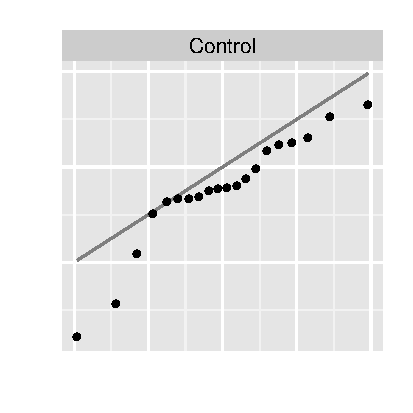
\includegraphics[width=0.3\textwidth]{qqplots1}
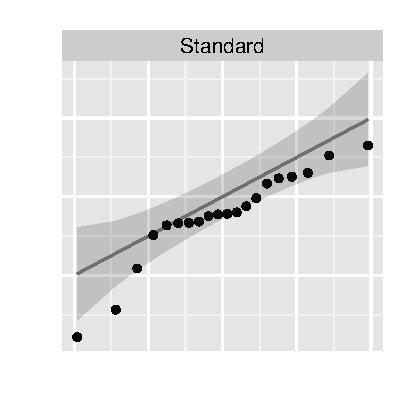
\includegraphics[width=0.3\textwidth]{qqplots2}
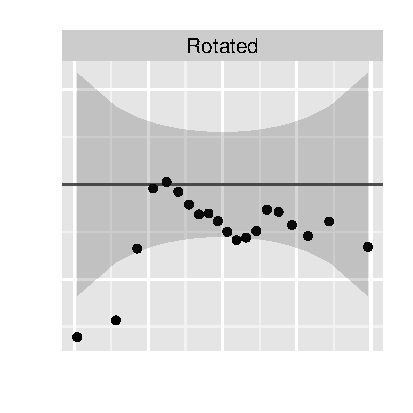
\includegraphics[width=0.3\textwidth]{qqplots3}
\caption{ \label{qqplots} Three versions of Q-Q plots: control, standard, and rotated.}
\end{figure}


Let $X_i \sim B_{1, \pi_i}, 1 \le i \le n$, where $X_i$ is the binary decision on the $i$th evaluation and $\pi_i$ is the probability with which the observer chooses the data plot. This probability is influenced by a number of factors:

\begin{center}
\begin{tabular}{lp{5in}}
$\tau$ & the design used in the lineup (Control, Standard, Rotated), \\
&  the specific parameters under which the data for the lineup were created: \\
&  $\delta$ \ \ \ degrees of freedom (2, 5, 10) {of the $t$ distribution} and \\
&  $\nu$  \ \ \ sample size (20, 30, 50, 75), \\
$d$ &  the level of difficulty based on the actual sample, and \\
$u$ & the users' subjective abilities.
 \end{tabular}
\end{center}
%
The combination of different levels of sample size and degrees of freedom of the $t$ distribution result in 12 parameter settings. Under each setting, we sampled data twice; additionally, we sampled two sets of null data for each sample, yielding 48 different sets of data, which we render in each of the variations, yielding 144 different lineups. 
Using  Amazon MTurk \citep{amazon}, 674 participants were each asked to evaluate ten different lineups each. 
\hh{weights? We dealt with multiple answers to lineups that offered this choice by using a weighting variabe with reciprocal values of the number of answers given by a participant.}
We model the probability of selecting the data plot from the lineup, $\pi$, with the help of model $M_1$:
\[
g(\pi_i) = \mu + \tau_{j(i)} +\delta_{k(i)}+ \nu_{s(i)} + u_{u(i)} + d_{d(i)}
\]
where $g$ is the logit link function, and $j(.), k(.), s(.), u(.)$, and $d(.)$ are all indexing functions that relate evaluation $i$ to the corresponding levels in the factor variables, to the observer, or a particular data sample. More specifically, $j(i) \in \{$Control, Standard, Rotated$\}$; $k(i) \in \{2,5,10\}$; $s(i) \in \{20, 30, 50, 75\}$; $u(i)$ maps to the participant's id of the $i$th evaluation and $d(i)$ identifies the particular data sample used for it. 

Both user ability, $u$, and sample difficulty, $d$, are modeled as independent, normally distributed  random effects, i.e. $u_{u(i)} \sim N(0, \sigma_u^2)$, $d_{d(i)} \sim N(0,\sigma_d^2)$ with cov$(u, d) = 0$.





\begin{figure}
\begin{subfigure}[b]{0.5\textwidth}
\begin{knitrout}
\definecolor{shadecolor}{rgb}{0.969, 0.969, 0.969}\color{fgcolor}
\includegraphics[width=\maxwidth]{figure/abilities} 

\end{knitrout}

\end{subfigure}
\begin{subfigure}[b]{0.5\textwidth}
\begin{knitrout}
\definecolor{shadecolor}{rgb}{0.969, 0.969, 0.969}\color{fgcolor}
\includegraphics[width=\maxwidth]{figure/abilities2} 

\end{knitrout}

\end{subfigure}
\caption{\label{fig:ranef}Histograms of random effects of individuals' abilities (left) and difficulty level of the data (right). }
\end{figure}

% latex table generated in R 3.1.0 by xtable 1.7-3 package
% Sun Aug  3 11:20:58 2014
% xtable(summary(m0)$coefficients, digits=c(0,2,3,2,4))
\begin{table}[ht]
\centering
\caption{\label{tab:model} Coefficients and significances corresponding to  model $M_1$. The type of design is important for the power of a lineup. Rotated Q-Q plots lose a significant amount of power compared to both the regular and the standard version of Q-Q plots. }
\begin{tabular}{rrrrrl}
  \hline
 &\bf Estimate &\bf Std. Error &\bf z value &\bf Pr($>$$|$z$|$) & \\ 
  \hline
  Intercept &  -5.37 & 0.769 & -6.98 & 0.0000  & *** \\ [3pt]
\multicolumn{3}{l}{\bf design} \\
   Control & 0.00 & ----- & ----- & ----- \\ 
   Standard & 0.06 & 0.103 & 0.62 & 0.5371 \\
   Rotated & -0.50 & 0.104 & -4.77 & 0.0000 & ***\\  [3pt]
\multicolumn{4}{l}{\bf degrees of freedom} \\
  2 & 6.63 & 0.752 & 8.82 & 0.0000 & ***\\ 
  5 & 2.65 & 0.732 & 3.61 & 0.0003 & **\\ 
  10 & 0.00 & ----- & ----- & ----- \\ [3pt]
\multicolumn{3}{l}{\bf sample size} \\
  20 & 0.00 & ----- & ----- & ----- \\ 
  30 & 0.88 & 0.848 & 1.03 & 0.3014 \\ 
  50  & 3.26 & 0.837 & 3.90 & 0.0001 & ***\\ 
  75 & 2.20 & 0.838 & 2.63 & 0.0086  & **\\ 
   \hline
\multicolumn{5}{l}{Signif. codes:  0 $\le$ *** $\le$ 0.001 $\le$ ** $\le$ 0.01 $\le$ * $\le$ 0.05 $\le$ . $\le$ 0.1 $\le$ ' ' $\le$ 1}
\end{tabular}
\end{table}

The estimated model coefficients for model $M_1$ are shown in Table~\ref{tab:model}. 
Estimates of the variance components are $\widehat{\sigma}_u = 0.44$, $\widehat{\sigma}_d=0.44$, and $\widehat{\sigma} = 0.31$. Variances of user ability and data difficulty are large relative to residual variance, indicating that both random effects are necessary.
%
As expected, the task of identifying non-normality is easier with increased sample size and more pronounced deviations from normality, as is the case with lower degrees of freedom. The  design of the Q-Q plot is of huge importance for the probability of choosing the data plot. Interestingly, the rotated version of the Q-Q plot is significantly less suitable for the task of assessing normality compared to the control. Additionally, adding confidence bands helps with evaluation, but not significantly. 

Note that none of the data plots in the lineups were actually created using data from a normal distribution. This should lead to rejection of the null hypothesis in every single instance. This is not quite true, as can be seen in Table~\ref{tab:reject}, but what also becomes evident is the high power  of visual inference. Based on lineups we are able to reject non-normality much more often than with any of the classical tests.

% latex table generated in R 3.0.1 by xtable 1.7-1 package
% Mon May 27 20:57:50 2013
\begin{table}[ht]
\centering
\caption{\label{tab:reject} 
Out of the 48 non-normal samples, 24 get rejected at the 5\% significance level based on evaluation by observers. None of the classical tests come close to that rejection rate. From left to right, we see the number of rejections from visual inference as well as the Anderson-Darling, Shapiro-Wilk, Cram\'er-von Mises and Kolmogorov-Smirnov tests for normality.}
\begin{tabular}{rrrrrr}
  \hline
Result & Visual & AD & SW & CVM & KS \\ 
  \hline
  reject & 24 & 10 & 16 &  8 & 10 \\ 
  not reject & 24 & 38 & 32 & 40 & 38 \\ 
   \hline
\end{tabular}
\end{table}






\begin{figure}
\centering
\begin{subfigure}[b]{.3\textwidth}
\begin{knitrout}
\definecolor{shadecolor}{rgb}{0.969, 0.969, 0.969}\color{fgcolor}
\includegraphics[width=\maxwidth]{figure/unnamed-chunk-1} 

\end{knitrout}

\end{subfigure}
\begin{subfigure}[b]{.3\textwidth}
\begin{knitrout}
\definecolor{shadecolor}{rgb}{0.969, 0.969, 0.969}\color{fgcolor}
\includegraphics[width=\maxwidth]{figure/unnamed-chunk-2} 

\end{knitrout}

\end{subfigure}
\begin{subfigure}[b]{.3\textwidth}
\begin{knitrout}
\definecolor{shadecolor}{rgb}{0.969, 0.969, 0.969}\color{fgcolor}
\includegraphics[width=\maxwidth]{figure/unnamed-chunk-3} 

\end{knitrout}

\end{subfigure}
\caption{\label{fig:compare}Proportions of successful evaluation of the same data in the three different variations of Q-Q plots. Standard and control displays exhibit the highest correlation. Rotated Q-Q plots agree with decisions made based on Q-Q plots in the control or standard design, but display lower rates of correct responses in the `middle' field.  }
\end{figure}

%------------------------------------------------------------------------------------
\section{Discussion}
%------------------------------------------------------------------------------------

\alnote{We can recap and discuss how we can extend the study (aspect ratio for the rotated plots, etc.)}

%------------------------------------------------------------------------------------
\section{Other material}
%------------------------------------------------------------------------------------



Similar to observations made in other lineup experiments (XXX cite Mahbub's socio paper), there is no indication of a `learning' effect within a participant's first ten answers (see figure~\ref{fig:attempts}), indicating that lineups make use of an inherent ability. The overall proportion of correct responses is very stable, fluctuating around 0.41. However, the variability observed is close to 0.5. What does change, is the time taken by participants to answer a lineup. From initially 53.6 seconds in the first answer, the response time drops to 33 seconds at the tenth evaluation.
\begin{figure}
\centering
\begin{subfigure}[b]{.5\linewidth}
\begin{knitrout}
\definecolor{shadecolor}{rgb}{0.969, 0.969, 0.969}\color{fgcolor}
\includegraphics[width=\maxwidth]{figure/fig1} 

\end{knitrout}

\end{subfigure}
\begin{subfigure}[b]{.5\linewidth}
\begin{knitrout}
\definecolor{shadecolor}{rgb}{0.969, 0.969, 0.969}\color{fgcolor}
\includegraphics[width=\maxwidth]{figure/fig2} 

\end{knitrout}

\end{subfigure}
\caption{\label{fig:attempts}Proportion of correct answers by attempt (left) and time taken in each of the first ten attempts (right). The proportion of correct responses stays constantfor successive attempts, while the time to answer decreases significantly over the same number of attempts.}
\end{figure}
\bibliographystyle{apalike}
\bibliography{qqplots}


\end{document}
